\documentclass{article}


\usepackage{arxiv}

\usepackage[utf8]{inputenc} % allow utf-8 input
\usepackage[T1]{fontenc}    % use 8-bit T1 fonts
\usepackage{hyperref}       % hyperlinks
\usepackage{url}            % simple URL typesetting
\usepackage{booktabs}       % professional-quality tables
\usepackage{amsfonts}       % blackboard math symbols
\usepackage{nicefrac}       % compact symbols for 1/2, etc.
\usepackage{microtype}      % microtypography
\usepackage{lipsum}

\usepackage{graphicx}

\title{Paper title}


\author{
  Juliana Y.~Rhee\\
  Center for Brain Science\\
  Department of Molecular and Cellular Biology\\
  Harvard University\\
  Cambridge, MA 02138 \\
  \texttt{rhee@g.harvard.edu} \\
  %% examples of more authors
   \And
 David D.~Cox \\
 Center for Brain Science\\
  Department of Molecular and Cellular Biology\\
  Harvard University\\
  Cambridge, MA 02138 \\
  \texttt{rhee@g.harvard.edu} \\
  %% \AND
  %% Coauthor \\
  %% Affiliation \\
  %% Address \\
  %% \texttt{email} \\
  %% \And
  %% Coauthor \\
  %% Affiliation \\
  %% Address \\
  %% \texttt{email} \\
  %% \And
  %% Coauthor \\
  %% Affiliation \\
  %% Address \\
  %% \texttt{email} \\
}

\begin{document}
\graphicspath{./figures/}

\maketitle

\begin{abstract}
Text text text
\end{abstract}


% keywords can be removed
\keywords{First keyword \and Second keyword \and More}


\section{Introduction}
The brain's visual system translates ambiguous and rapidly-changing patterns of light falling on the retina into a coherent representation of the external world that can be used to guide behavior. The hierarchical organization of sensory cortex is thought to play a key role in its ability to extract and learn about latent structure from visual inputs. For example, visual object recognition in primates is thought to emerge through sequential processing across cortical areas in the ventral visual pathway~\cite{rustselectivity2010, DiCarlo:2007aa, dicarlo2012does, Chen2014682}, and numerous studies show increasing selectivity for complex stimuli at progressively higher levels of a sensory processing hierarchy~\cite{desimone1984stimulus, logothetis1996visual}. 

Similarly, learning produces distinct changes across the visual cortical hierarchy in a stimulus-specific and task-dependent way. For example, neural responses to task stimuli are specifically enhanced in inferotemporal cortex (IT), the highest level of the ventral path, after monkeys learn to discriminate complex shapes~\cite{kobatake1998shape, sigalavisual2002}. Other studies show changes in lower level areas, such as V1 or V4~\cite{schoupspractising2001, raiguellearning2006, ghose2002physiological, vogelsdoes1994} when simpler stimuli are used, as in orientation discrimination tasks. In all cases, perceptual learning results in specific changes in neural representations~\cite{goldstone1998perceptual, fine2002comparing, OpdeBeeck201022}. However, the nature of the transformations that occur from one level of the hierarchy to the next remain poorly understood. 


\section{Retinotopic organization of rat visual cortex}
\label{sec:retinotopy}

Text goes here.

\subsection{Macroscopic organization}
Text text text.

\begin{figure}[ht]
  %\centering
  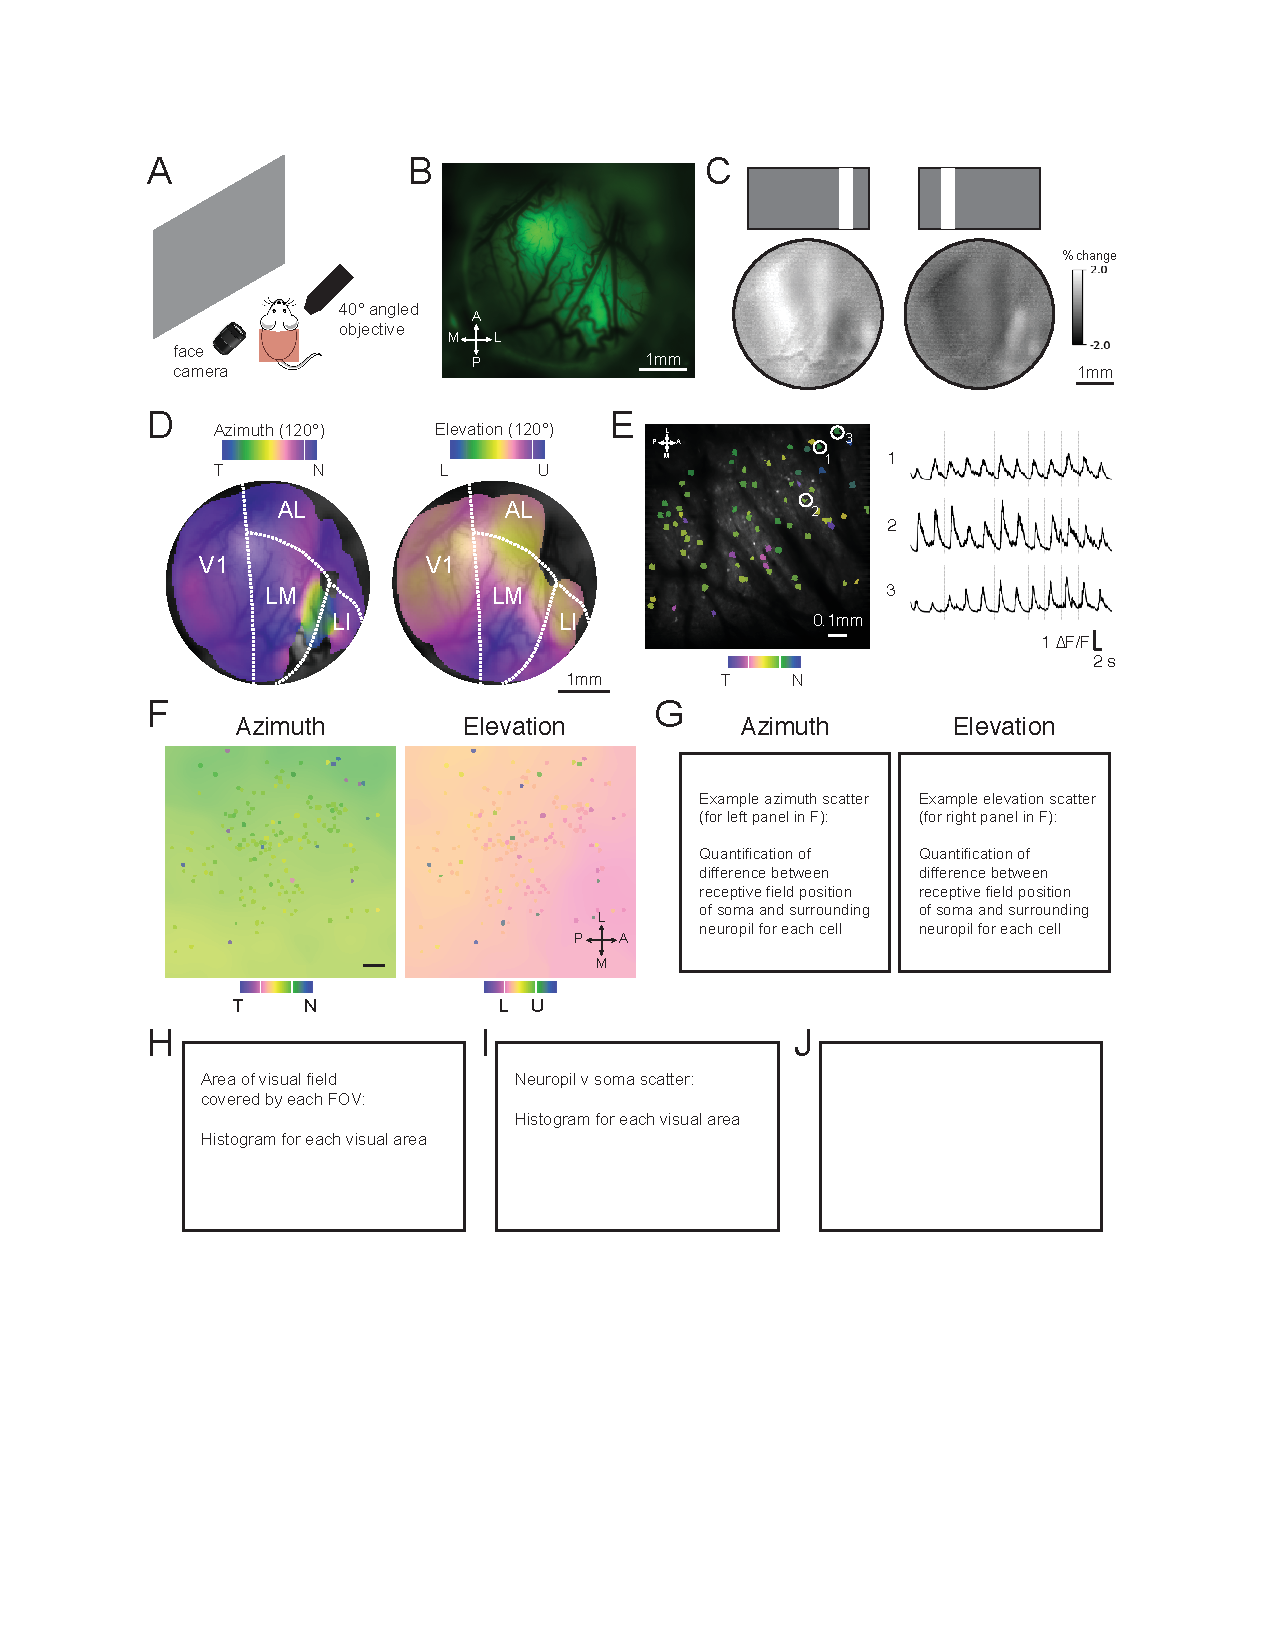
\includegraphics[width=\textwidth]{figures/retino.pdf}
  \caption{Macroscopic retinotopic organization in rat visual cortex.}
  \medskip
  \small
  A.  Experiment setup.  
  B.  Epifluorescence image of an example cranial window with AAV9-GCaMP6f expression. Scale bar is 1mm.  
  C.  GCaMP6f response to a vertically-oriented moving bar. \textit{Left}: Average response to a 5 degree vertical bar on the animal’s nasal visual field (upper inset). \textit{Right}: Average response to a 5 degree vertical bar presented on the animal’s temporal visual field (upper inset). 
  D.  Pseudo-colored maps of the cranial window shown in C for azimuth (\textit{left}) and elevation (\textit{right}). Outlined visual areas:  V1 (primary visual cortex), LM (lateral-medial), LI (lateral-intermediate), AL (antero-lateral). N=nasal visual field, T=temporal visual field. 
  E.  Retinotopic map of two-photon field of view.  \textit{Left}: Average two-photon image of visually-evoked responses to a rightward moving bar stimulus.  Cells are color-coded by azimuth position. N=nasal, T=temporal.  \textit{Right}:  Average time-courses across 4 repetitions of the rightward moving bar for the circled cells. 
  F.  Maps of retinotopic preference for azimuth (\textit{right}) and elevation (\textit{left}).  Cells are color-coded by position in azimuth or elevation.  All other pixels contain a smoothed estimate of neuropil retinotopic preferences. N=nasal, T=temporal.
  G.  Difference between each cell’s retinotopic preference and its surrounding neuropil for the maps shown in F. \textit{Left}:  Retinotopic scatter along azimuth. \textit{Right}:  Retinotopic scatter along elevation.
  H.  Areal of visual field coverage for each two-photon FOV for visual area V1, LM and LI. 
  I.  Degree of retinotopic scatter for all FOVs recorded in each visual area.
  J.  unknown
  \label{fig:fig1}
\end{figure}

\subsubsection{Retino finding 1}
Text text. 

\subsubsection{Retino finding 2}
Text text. 



\subsection{Receptive field properties in rat visual cortex}
Text text text.


\subsubsection{RF section 1}
Text text text
See Figure \ref{fig:fig2}.

\begin{figure}[ht]
  %\centering
  \includegraphics[width=\textwidth]{figures/receptivefields.pdf}
  \caption{Microscale organization and receptive field properties of rat visual cortex.}
  \medskip
  \small
  A.  \textit{Left}:  PSTHs arranged by stimulus position for three example cells in V1. \textit{Right}:  Receptive fields estimated from 2d-Gaussian fits for all cells in a V1 FOV.
  B.  \textit{Left}:  PSTHs arranged by stimulus position for three example cells in LI. \textit{Right}:  Receptive fields estimated from 2d-Gaussian fits for all cells in a LI FOV.
  C.  Receptive field centers as a function of cortical position along the azimuth axis. Blue: Receptive field center estimated from 10 repetitions at each position. \textit{Black}: Bootstrapped estimates of receptive field centers (vertical error bars show 95\% CI, horizontal markers show median of bootstrap distribution of azimuth position). \textit{Red}: Linear regression (shaded area shows 95\% CI).
  D.  Slope of linear regression of cortical position on receptive field position for visual areas V1, LM, and LI for azimuth (\textit{left}), elevation (\textit{middle}), and the average absolute values of azimuth and elevation conditions (\textit{right}). Data points show the measured slope for each FOV.  Boxes show quartile range for each visual area, whiskers show the remainder of the distribution.
  E.  Pairwise-distances in cortical space as a function of receptive field distance for V1, LM, and LI. Box plots as in D. 
  F.  Cumulative distribution of average receptive field sizes for V1, LM and LI  Average combines major and minor axes of fit receptive fields. 
  G.  Percent of receptive field overlap in V1, LM and LI.  
  H.  Distributions of correlations between cortical distance and stimulus condition for all pairs of neurons within each visual area. 

  \label{fig:fig2}
\end{figure}

\subsubsection{RF section 2}
Text text text

\section{Feature tuning in rat visual cortex}
text intro here

\subsection{Features section 1}
text text text

\begin{figure}[ht]
  %\centering
  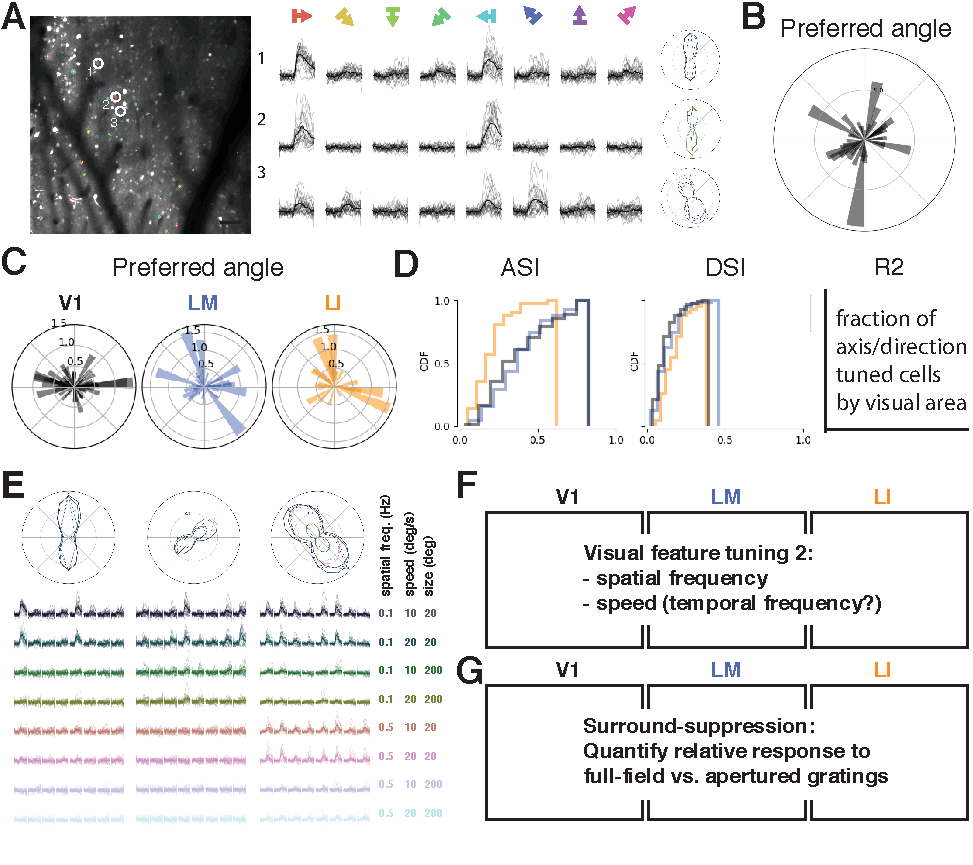
\includegraphics[width=\textwidth]{figures/features.pdf}
  \caption{Feature tuning.}
  \medskip
  \small
  A.  \textit{Left}:  Two-photon image of responses to drifting grating stimuli with cells masked by preferred angle. \textit{Middle}:  Responses to 20 presentations of drifting gratings for the three cells circles on the left. Thicker lines show average trace. \textit{Right}:  Corresponding tuning curves fit to responses shown in the middle. 
  B.  Distribution of preferred direction for tuned cells in the example FOV shown in A (see methods).
  C.  Distribution of preferred direction for  tuned cells collapsed across FOVs for V1, LM and LI (see methods).
  D.  \textit{Left}: Fraction of tuned cells out of all visually responsive cells by area (see methods). Boxes show inter-quartile (IQR) range, whiskers extend 1.5*IQR. Cumulative distribution of axis-selective (\textit{middle}) and direction-selective (\textit{right}) indices by visual area. 
  E.  Responses to oriented gratings across different stimulus configurations from three example cells. \textit{Top}: For each cell, polar plots of raw (dotted lines) and fit (solid) orientation tuning for the subset of conditions that passed fitting metrics (see methods). \textit{Bottom}: For each cell, traces represent trials for each grating direction, colors and rows represent the stimulus configuration denoted at the right of each row.
  F.  Spatial frequency and temporal frequency preferences by visual area.
  G.  Tuning modulation by stimulus size.
  H.  Tuning similarity as a function of cortical distance.  Aggregate metrics across datasets for each visual area.
  I.  Distributions of correlations between cortical distance and stimulus condition for all pairs of neurons within each visual area. 
  J.  Averages of the upper triangle of trial-to-trial correlation matrices for pairs of visually responsive cells. Each point in each matrix is the correlation between two cells’ response vectors, composed of the cell’s mean stimulus response for each trial. Each data point shows the upper-triangle average for one FOV.
  \label{fig:fig3}
\end{figure}

\subsection{Features section 2}
text text text
See Figure \ref{fig:fig3}.


\section{Object preference in rat visual cortex}
text intro here

\subsection{Objects section 1}
text text text

\begin{figure}[ht]
  %\centering
  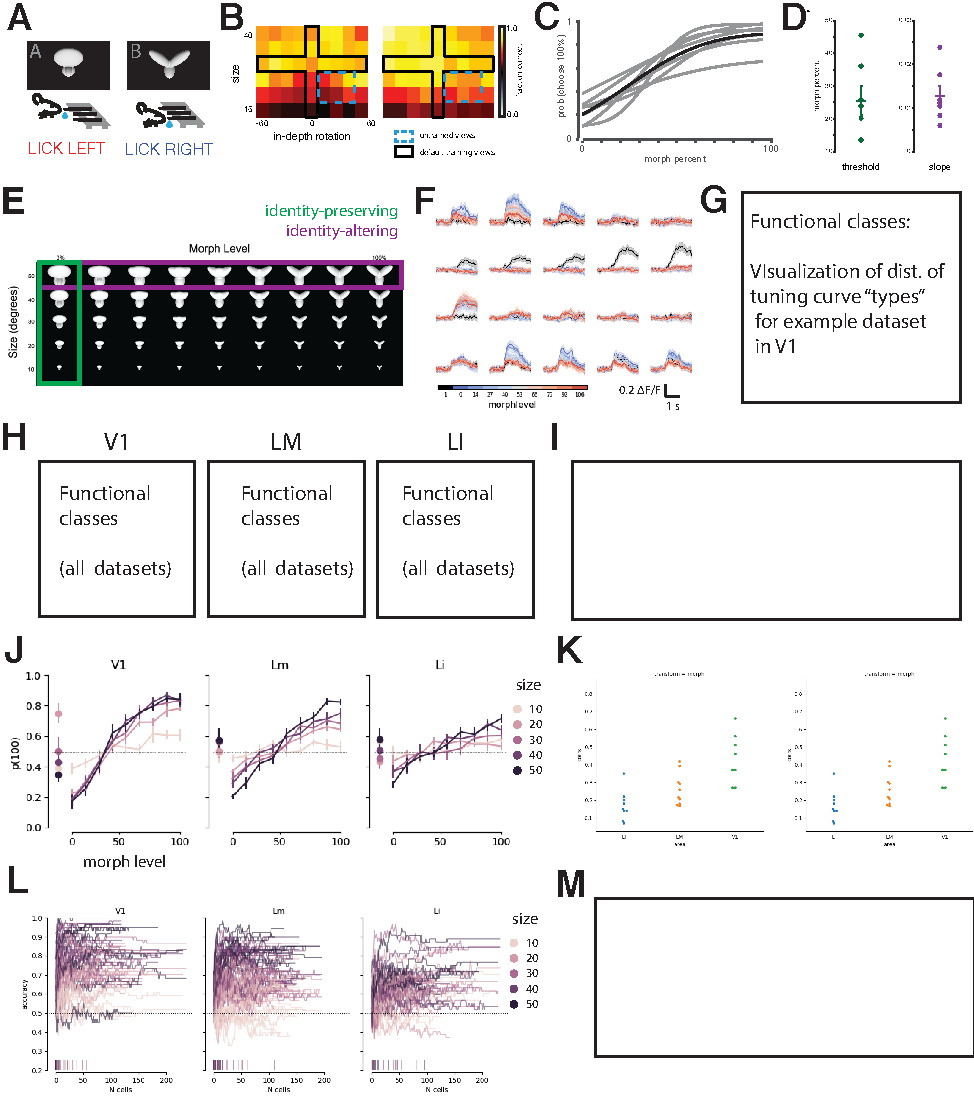
\includegraphics[width=\textwidth]{figures/objects.pdf}
  \caption{Object tuning.}
  \medskip
  \small
  A.  Schematic of stimulus conditions.
  B.  Responses of eight different cells representing four example functional classes.  Each row shows two examples of:  1)  Morph-tuned, size-tolerant, 2)  Luminance-tuned only, 3) Size-tuned only, 4)  Morph- and size/luminance-tuned. Traces show mean response (+/- sem) across repetitions for each stimulus condition.
  C.  Visualization of functional class clusters for example dataset.
  D.  Quantification of functional class distributions by visual area.
  E.  Analysis of the linearity of the relationship between neural responses and object features.  \textit{Left}:  Linear regression on size for example FOV. Each point shows the predicted size versus the actual size of the stimulus presented on a trial. Shade of blue denotes which morph was presented on that trial.  \textit{Middle}:  Linear regression on morph. Points and colors as in the left panel.  \textit{Right}:  Relationship between regression coefficients for morph and for size. Each data point is a cell. Lack of correlation suggests different functional sub-populations contribute to size and morph decoding.
  F.  Linear readout of size and morph by visual area. Each data point is the correlation between the predicted vs true values for one FOV, as shown in the example regressions in the left and middle panels of E.  \textit{Left}:  Pearson’s correlation between predicted and true values for size regression.  \textit{Right}:  Pearson’s correlation between predicted and true values for morph regression. 
  G.  Trial-to-trial correlations between pairs of visually responsive cells for one example FOV in each of V1, LM and Li. Each point in a matrix is the correlation between two cells’ response vectors, composed of the cell’s mean stimulus response for each trial. a
  H.  Average of the upper triangle of the correlation matrix for each FOV, by visual area. Each data point is the average for one FOV. 
  \label{fig:fig4}
\end{figure}

\section{Models of object classification}
text intro here

\subsection{All stim section 1}
text text text

\begin{figure}[ht]
  %\centering
  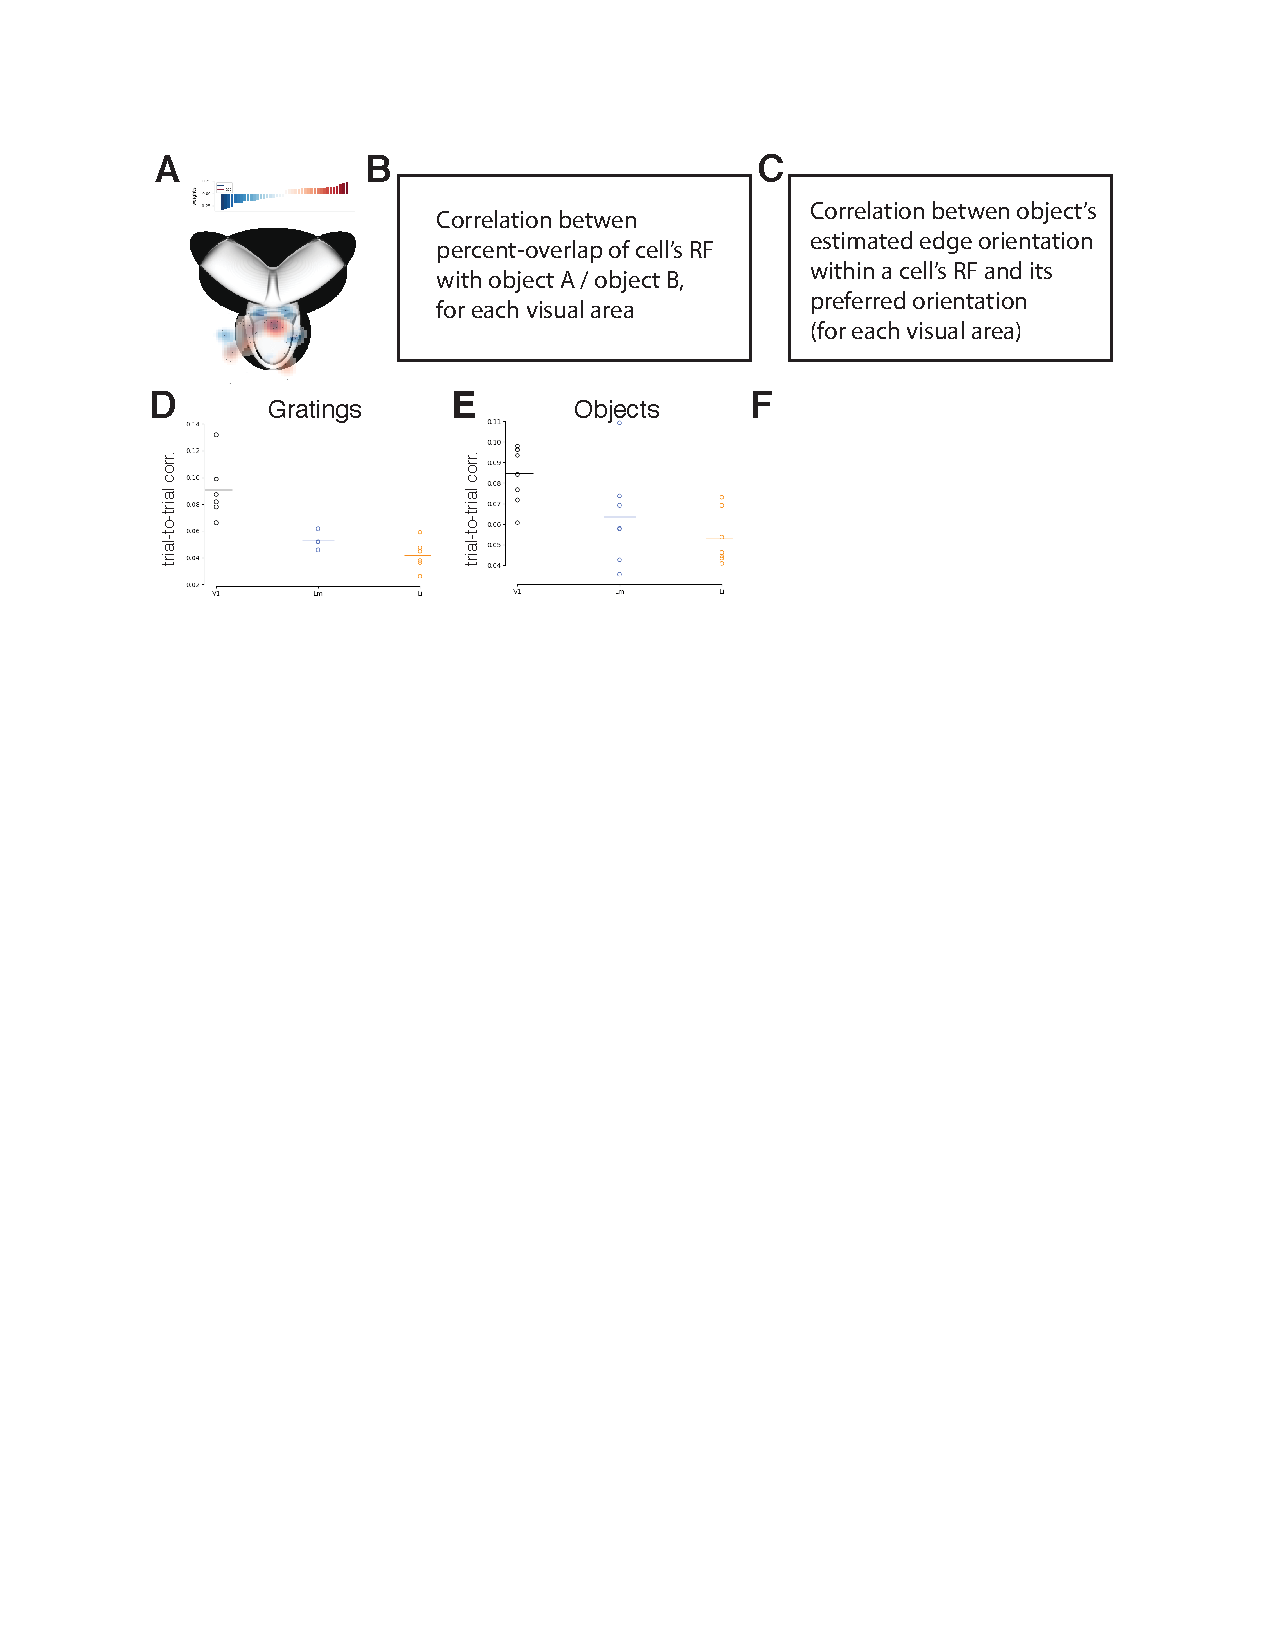
\includegraphics[width=\textwidth]{figures/allstim.pdf}
  \caption{Models for classification choices.}
  \medskip
  \small
  legend text here
  \label{fig:fig5}
\end{figure}

\subsection{All stim section 2}
text text text

\subsection{All stim section 3}
text text text



\section{Appendix}

\begin{table}
 \caption{Sample table title}
  \centering
  \begin{tabular}{lll}
    \toprule
    \multicolumn{2}{c}{Part}                   \\
    \cmidrule(r){1-2}
    Name     & Description     & Size ($\mu$m) \\
    \midrule
    Dendrite & Input terminal  & $\sim$100     \\
    Axon     & Output terminal & $\sim$10      \\
    Soma     & Cell body       & up to $10^6$  \\
    \bottomrule
  \end{tabular}
  \label{tab:table}
\end{table}


\subsection{Tables}
Stuff here.
See awesome Table~\ref{tab:table}.

\subsection{Supplementary Figures}
\begin{itemize}
\item related to Figure \ref{fig:fig1}.
\item related to Figure \ref{fig:fig3}.
\item related to Figure \ref{fig:fig4}.
\end{itemize}


\bibliographystyle{unsrt}  
%\bibliography{references}  %%% Remove comment to use the external .bib file (using bibtex).
%%% and comment out the ``thebibliography'' section.


%%% Comment out this section when you \bibliography{references} is enabled.
\begin{thebibliography}{1}

\bibitem{kour2014real}
George Kour and Raid Saabne.
\newblock Real-time segmentation of on-line handwritten arabic script.
\newblock In {\em Frontiers in Handwriting Recognition (ICFHR), 2014 14th
  International Conference on}, pages 417--422. IEEE, 2014.

\bibitem{kour2014fast}
George Kour and Raid Saabne.
\newblock Fast classification of handwritten on-line arabic characters.
\newblock In {\em Soft Computing and Pattern Recognition (SoCPaR), 2014 6th
  International Conference of}, pages 312--318. IEEE, 2014.

\bibitem{hadash2018estimate}
Guy Hadash, Einat Kermany, Boaz Carmeli, Ofer Lavi, George Kour, and Alon
  Jacovi.
\newblock Estimate and replace: A novel approach to integrating deep neural
  networks with existing applications.
\newblock {\em arXiv preprint arXiv:1804.09028}, 2018.

\end{thebibliography}


\end{document}
